\documentclass[12pt,]{article}
\usepackage[utf8]{inputenc}
\usepackage[T1]{fontenc}
\usepackage{mathptmx}
\usepackage{geometry}
\usepackage{mathtools}
\usepackage[english]{babel}
\usepackage{graphicx}
\usepackage{stackengine}
\usepackage[os=win]{menukeys}
\usepackage{hyperref}
\usepackage{minted}
\usepackage{xcolor}
\usepackage{tikz}
\usepackage[yyyymmdd,hhmmss]{datetime}
\usepackage{etoolbox}
\usepackage[inline]{enumitem}
\usepackage[figurename=Gambar-]{caption}

\patchcmd{\thebibliography}{\section*{\refname}}{}{}{}

\addto\captionsenglish{\renewcommand{\contentsname}{Daftar Isi}}

\hypersetup{
	colorlinks=true, %set true if you want colored links
	linktoc=all,     %set to all if you want both sections and subsections linked
	linkcolor=blue,  %choose some color if you want links to stand out
	urlcolor=blue,	 %url color
}

\geometry{
	a5paper,
	left=15mm,
	right=10mm,
	top=10mm,
	bottom=15mm,
}

\title{\Large \bf
	Quick Usage Manual\\
}

\author{Achmadi ST MT}

\date{}

\hypersetup{citecolor=black}

\definecolor{LightGray}{gray}{0.95}

\begin{document}
	\maketitle
	\thispagestyle{empty}
	
	\vspace*{300pt}
	
	Update: {\today} at \currenttime \\
	
	%%%%%%%%%%%%%%%%%%%%%%%%%%%%%%%%%%%%%%%%%%%%%%%%%%%%%%%%%%%%%%%%%
	
	\newpage
	\tableofcontents
	
	%%%%%%%%%%%%%%%%%%%%%%%%%%%%%%%%%%%%%%%%%%%%%%%%%%%%%%%%%%%%%%%%%
	
	\newpage
	\section{Pendahuluan}
	
	Berikut beberapa poin pendahuluan yang selayaknya diperhatikan sebelum penggunaan.
	
	\subsection{Antarmuka}
	
	Berikut ilustrasi antar muka unit Audiometri (untuk selanjutnya disebut Unit saja):
	
	\begin{figure}[!ht]
		\centering
		\includegraphics[width=300pt]{images/part}
		\caption{Antar muka Unit}
	\end{figure}

	\newpage
	\textbf{Keterangan:}
	\begin{enumerate}
		\item Power Switch untuk ON/OFF Unit.
		\item Jack 3.5mm untuk Ouput Nada Murni.
		\item LED Merah (Indikator Jawaban Salah).
		\item Grup LED Kuning (Indikator Pilihan Jawaban).
		\item Grup Tombol Pilihan Jawaban.
		\item Port USB untuk Charging.
		\item LED Hijau (Indikator Jawaban Benar).
		\item LED Biru (Indikator Mode Unit).
		\item Tombol Reset untuk memulai ulang Unit.
		\item Slot Micro SDCard untuk penyimpanan.
		\item Port USB untuk Data dan Setting.
	\end{enumerate}
	
	\subsection{Charging}
	
	Untuk Charging, dapat menggunakan adaptor charger and kabel microUSB yang umum digunakan untuk mengisi daya perangkat Android.
	
	Pastikan Unit dalam \textbf{kondisi mati/OFF} saat charging. 
	Sambungkan Unit ke adaptor dengan kabel microUSB pada port nomer 6 di gambar-1. Kemudian sambungkan adaptor ke sumber AC/PLN.
	
	Unit akan menampilkan nyala \textbf{Merah} pada port USB Charging.
	Tunggu nyala tersebut berubah menjadi \textbf{Biru} sebagai tanda telah penuh.
	
	\newpage
	\section{Persiapan}
	
	\subsection{Cek Persiapan}
	
	Sebelum menghidupkan, pastikan beberapa hal berikut:
	
	\begin{itemize}
		\item Unit tidak sedang terhubung kabel-USB apapun.
		\item Micro-SDcard format FAT32 telah terpasang.
		\item Headphone yang tersedia telah terhubung Unit.
		\item Headphone telah terpakai di pengguna dan tidak terbalik
		kanan dan kiri.
	\end{itemize}

	\subsection{Menyalakan}
	
	Untuk menyalakan, perhatikan ilustrasi berikut:
	
	\begin{figure}[!ht]
		\centering
		\includegraphics[width=300pt]{images/turnon}
		\caption{Menyalakan Unit}
	\end{figure}
	
	\newpage
	Urutan menyalakan Unit:
	\begin{itemize}
		\item Geser Power Switch (no.1).
		\item LED Biru no.2 akan menyala.E
		\item LED no. a, b, c, d, dan e akan menyala bergantian.
		\item Tone akan terdengar 2x kiri dan kanan bergantian dari port Audio (no.3)
		\item LED Biru no.2 menjadi berkedip.
	\end{itemize}

	Jika respon Unit tidak seperti di atas saat pertama dinyalakan, maka Unit sedang tidak layak pakai
	
	\subsection{LED Indikator Biru}
	
	LED Indikator Biru adalah LED no.8 pada gambar-1, atau no.2 pada gambar-2.
	
	Berikut adalah arti dari pola berkedip LED Biru:
	\begin{itemize}
		\item Berkedip lambat.\\
		Unit dalam kondisi Idle dan siap dipakai.
		
		\item Berkedip 2x cepat dan mati dalam selang waktu.\\
		Micro-SDcard tidak dapat diakses atau tidak ada.
		
		\item Berkedip cepat.\\
		Sedang dalam sesi proses Audiometri.
		
		\item Tidak Berkedip.\\
		Unit mengalami freeze/hank. Tekan tombol Reset atau nyalakan ulang Unit.
	\end{itemize}
	
	\newpage
	\section{Audiometri}
	
	\textbf{Perhatian:} Untuk bab panduan ini, sebaiknya dipahami terlebih dahulu sebelum dipraktikan.
	
	\subsection{Memulai}
	Berikut cara memulai sesi Audiometri:
	
	\begin{figure}[!ht]
		\centering
		\includegraphics[width=300pt]{images/Start}
		\caption{Memulai Audiometri}
	\end{figure}

	\begin{itemize}
		\item Tekan tombol A, LED di no.1 akan menyala.
		\item Tekan tombol B, LED di no.2 akan berganti menyala.
		\item Tekan tombol C, LED di no.3 akan berganti berkedip cepat.
		Proses Audiometri dimulai.
	\end{itemize}
	
	\newpage
	\subsection{Sesi Audiometri}
	
		\begin{figure}[!ht]
		\centering
		\includegraphics[width=300pt]{images/sesi}
		\caption{Memulai Audiometri}
	\end{figure}
	
	Berikut interaksi saat sesi proses Audiometri:
	\begin{enumerate}
		\item LED Kuning pada baris 1 akan menyala bergantian.
		\item Nada akan terdengar pada salah satu LED Kuning tersebut.
		\item Tekan salah satu tombol di grup no.3 dimana LED menyala bersamaan dengan terdengar bunyi nada murni.
		\item LED Merah atau Hijau akan menyala tergantung salah/benar jawaban
		\item Proses Sesi Audiometri selesai saat LED Indikator Biru (no.5) berubah berkedip lambat.
	\end{enumerate}

	\newpage
	\section{Spesifikasi Teknis}
	Berikut spesifikasi teknis unit box Audiometri Portable:
	
	\begin{enumerate}
		\item Tegangan Kerja: VDD (2.5v - 4.2v)
		\item USB Charging: VCC (4.5v - 5.5v)
		\item Dimensi: mm X mm
		\item Berat: gram
		\item Minimal Impendance: 300 $\Omega$
		\item Frekuensi Nada Murni: 250 Hz - 8000 Hz
		\item Loudness Nada Murni: 35 dB(SPL) - 85 dB(SPL)
		\item USB Data: protokol STM32-VCP
		\item IoT Port: Wi-Fi Client
		
	\end{enumerate}
	
\end{document}